\documentclass[conference]{IEEEtran}
\IEEEoverridecommandlockouts
% The preceding line is only needed to identify funding in the first footnote. If that is unneeded, please comment it out.
\usepackage{cite}
\usepackage{url}
\usepackage{fancyvrb}
\usepackage[svgnames]{xcolor}
\usepackage{graphicx, float}
\usepackage{amsmath,amssymb,amsfonts}
\usepackage{algorithmic}
\usepackage{graphicx}
\usepackage{textcomp}
\usepackage{xcolor}

\graphicspath{{Figures/}}
\def\BibTeX{{\rm B\kern-.05em{\sc i\kern-.025em b}\kern-.08em
    T\kern-.1667em\lower.7ex\hbox{E}\kern-.125emX}}
\begin{document}

\title{Research Paper: Cyberattack Case Study \\CIS 3360-Security in Computing\\Fall 2025\\
{\footnotesize Instructor: Jie Lin, Ph.D.}
\thanks{}
}

\author{{ Derek Oliveira}\\
\IEEEauthorblockA{\textit{department of engineering and computer science} \\
Orlando, United States of America \\
de937084@ucf.edu}
}

\maketitle

\begin{abstract}
The SolarWinds cyber breach, disclosed in December 2020, stands as one of the most significant cyber-espionage
incidents of the modern era. Through a sophisticated supply-chain compromise of SolarWinds' Orion platform, 
the state sponsored hacker group NOBELIUM gained persistent and covert access to U.S. government agencies,
corporations, and critical service providers. This paper examines the historical context, motives, and technical execution
of the attack that gave persistent anonymous access to SolarWinds' build environment, dubbed SUNBURST, demonstrating how the breach not 
only infiltrated high level networks but also undermined global trust in software ecosystems. By analyzing
NOBELIUM's tactics and the far-reaching consequences of the intrusion, I argue that the SolarWinds incident
represents a makeup call moment in cybersecurity. It highlights the vulnerability of supply chains, exposes
the limitations of traditional defense mechanisms, and guided us to new industry standards that shape the cybersecurity
landscape today. 
\end{abstract}

\begin{IEEEkeywords}
SUNBURST, formatting, style, styling, insert
\end{IEEEkeywords}

\section{Introduction}

% Identify the attack, when/whom it affected, why it meets the significance 
% criteria, your thesis, and a brief roadmap.

On December 13, 2020, SolarWinds, A Texas based technology company that develops network monitoring and IT 
infrastructure management software, announced what would become the most consequential cyber intrusion in history.
The breach focused on exploiting their Orion software, SolarWinds' main network monitoring platform used by U.S. 
government agencies, defense contractors, Fortune 500 corporations, and critical national service providers. 
The attackers, latter dubbed NOBELIUM by Microsoft's Threat Intelligence center (MSTIC) discovered to be
state sponsored attacker group backed by Russia, pursued espionage rather than economic gains.
SolarWinds itself was not the ultimate target, thou. Instead, its compromised software supply chain became the conveyor belt for malicious 
code that infiltrated networks of its customer base undetected for over a year. There were many exploits deployed in this attack, but for the 
scope of this research I will focus on the "SUNBURST" exploit.

By the time the intrusion was detected, NOBELIUM had already guaranteed their persistent, undetected access to email servers,
sensitive repositories, and classified communications for about one year. What followed was not a simple data breach, but a calculated and methodical 
campaign of cyber-espionage that exploited trust and used it as a mask for malicious intent. The SolarWinds incident was deemed a 
significant cyberattack not only because of its scale and sophistication, but also because of the national security risk it posed and 
the trust it shattered in the global technology leaders that are the watchdogs of our virtually connected world.

I argue that the SolarWinds breach represents a turning point in cybersecurity. It revealed the vulnerabilities of software supply 
chains, exposed the weakness of existing detection systems, and forced governments and corporations to rethink the resilience of their 
networks and how they can restructure themselves for reduced impact. To explore this claim, I will first outline the historical 
background and motives of NOBELIUM, then examine the technical methods of the SUNBURST intrusion, followed by an analysis of the attack's distinct 
features, its broader geopolitical implications and if the attack's patterns are still in use today. Finally, I will evaluate the lessons 
learned and how this incident reshaped modern approaches to cyber defense.


\section{Background}
%History of Development (actor/group, prior incidents, sponsorship, timeline) 
%and Purpose & Motivation (financial, political, espionage, disruption).
\subsection{NOBELIUM}
NOBELIUM, or as they were previously known; APT29/UNC2452/Cozy Bear/Midnight Blizzard/The Dukes,
is a Russian based threat actor attributed by the U.S. and European leaders as the foreign
intelligence service of the Russian Federation\cite{Microdoft2024NOBELIUM}. NOBELIUM can be traced back
to 2013, when European and American ministries of foreign affairs reported data breaches and theft of data 
through an incident that was latter named "Operation Ghost."\cite{MITREFirstNOBELIUMAttack} NOBELIUM is known for manipulating trust
withing security systems, falsifying digital certificates, virtually impersonating IT managers, and distorting security protocols
to reach their goals. These operations and tactics demonstrated NOBELIUM's strategic focus on infiltrating
high value targets and securing long-term access to sensitive information.\\

\subsection{History of Development}
The SolarWinds campaign unfolded over an extended timeline, as illustrated in Fig. \ref{fig:Timeline-of-Solorigate-attacks}. Initial 
reconnaissance and infiltration of SolarWinds’ infrastructure began as early as September 4, 2019,when NOBELIUM quietly embedded itself 
into the company’s software build process. By September 12, 2019, malicious test code had been injected into SolarWinds’ servers without
 detection, allowing the attackers to gather critical data and refine their ultimate payload, SUNBURST.\cite{MicrosoftDeepDiveSOLORIGATE}
\begin{figure}[H]
    \centering
    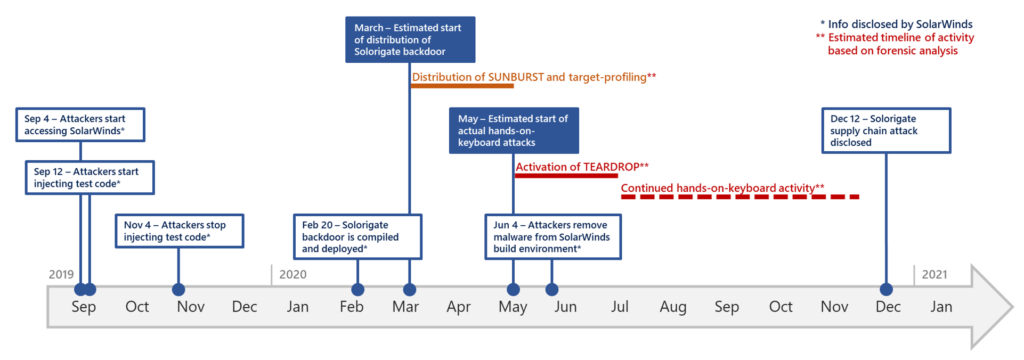
\includegraphics[width=3.4in]{Timeline-of-Solorigate-attacks.png}
    \caption{Image created by the MSTIC team on the timeline of events that led to the discovery of the SolarWinds
    breach.\\Source: \cite{MicrosoftDeepDiveSOLORIGATE} }
    \label{fig:Timeline-of-Solorigate-attacks}
\end{figure}

On February 20, 2020, NOBELIUM compiled a stable build of SUNBURST and deployed it within SolarWinds’ build environment. The malware was 
designed to lie dormant, waiting for legitimate Orion software updates to be compiled before injecting its backdoor code. This ensured that 
once updates were distributed, thousands of unsuspecting customers—including U.S. government agencies and major corporations—would unknowingly 
install compromised versions of Orion. By March 2020, this supply-chain compromise had effectively created persistent, stealthy backdoors across 
SolarWinds’ global customer base.\cite{MicrosoftDeepDiveSOLORIGATE}

Two months later, NOBELIUM expanded its operations by deploying TEARDROP, a custom loader for Cobalt Strike, against selected high-value targets.
 This allowed the attackers to escalate privileges, move laterally, and prepare for their true objectives with minimal detection. On June 4, 2020, 
 they removed all traces of malware from SolarWinds’ build environment, an act that further obscured their presence and erased forensic evidence.
  At this stage, no indicators of compromise remained within SolarWinds’ infrastructure, leaving investigators with few clues.\cite{MicrosoftDeepDiveSOLORIGATE}

For months afterward, “hands-on-keyboard” activity persisted, as NOBELIUM conducted real-time surveillance, extracted sensitive documents, and engaged 
in credential theft across infiltrated networks. Their covert campaign continued largely unnoticed until December 12, 2020—more than a year after initial 
access—when SolarWinds publicly disclosed the breach of its Orion software and the unprecedented compromise of its customers’ systems.\cite{MicrosoftDeepDiveSOLORIGATE}



\subsection{Purpose and Motivation}
Unlike cybercriminal groups motivated primarily by financial gain\cite{CoreTech2022Motivations}, NOBELIUM's campaign was politically driven. Its purpose was espionage, not profit. By exploiting SolarWinds'
trusted softare supply chain, the group gained covert entry into U.S. government agencies, including the department of homeland security, the Treasury department, and parts of the
pentagon, as well as major corporations in technology and critical infrastructure. The Intelligence collected had potential value for strategic leverage, diplomatic advantages, and technological competition.
\\
The motivations behind the breach align with Russia's broader geopolitical startegy of undermining adversaries, gathering intelligence, and projecting power in the digital domain\cite{HakalaMelnychuk2021RussiaCyberStrategy}.
By compromising secure communications, source code repositories, and decision-making processes, NOBELIUM not only accessed state secrets but also eroded confidence in the security of the west's digital
infrastructure. The attack represents a clear departure from disruptive cyber incidents, instead embodying a long term, covert infiltration campaign designed to maximize intelligence while minimizing detection.




\section{Analysis}
%Intended Usage Domain & Penetration Strategy 
%(industry/target environment, initial access, TTPs) 
%and Distinctive Features (innovations, what made it effective/different).
\subsection{Overview of SUNBURST (S0559)}
SUNBURST (MITRE S0559) was a trojanized component of SolarWinds' Orion platform that was compiled into
signed product updates and distributed to customers, as noted in figure \ref{fig:SUNBURSTPath}. Because the malicious code was delivered inside through vendor signed updates, it bypassed many integrity and whitelist checks
and achieved wide, trusted distribution. The implant combined application-layer mimicry, protocol obfuscation, and context-aware activation logic to remain dormant and undetected
until it found valuable execution environment.
\begin{figure}[H]
    \centering
    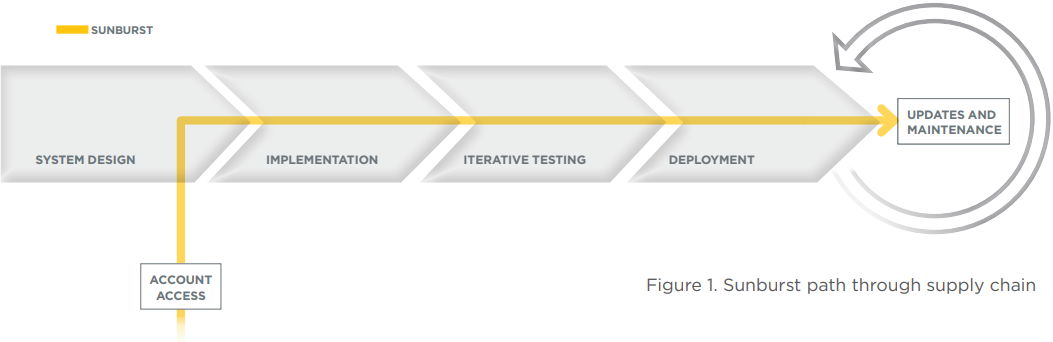
\includegraphics[width=3.4in]{SUNBURST-path.png}
    \caption{Source: \cite{BrokenTrustHerrEtAl} }
    \label{fig:SUNBURSTPath}
\end{figure}

\subsection*{Intended Usage Domain and Penetration Strategy}
SUNBURST targeted the software supply chain rather than a particular target. It's vehicle was the Orion legitimate updates, which gave it reach into federal civilian agencies,
parts of the intelligence and defense communities, major tech firms, and critical infrastructure operators that installed Orion for network monitoring. Environments where trusted
vendor updates are accepted and administrators grant monitoring software broad visibility and privileges.
\subsubsection{Initial Access}
trojanized build artifact
\begin{itemize}
    \item Vector: Compromise of SolarWinds' CI/Build environment to insert malicious code into the Orion build through the masking of a legitimate dll file(SolarWinds.Orion.Core.BusinessLayer.dll).
    The malicious file was then digitally signed and released as part of a legitimate update.\cite{MicrosoftDeepDiveSOLORIGATE}\\
    \item Dormancy and environment checks: After installation, SUNBURST employed time delays, execution-context filtering, and logic to avoid activating in low value environments.
    It performed checks against its command and control(C2) routines, minimizing the risk of noisy execution that could trigger detection.\cite{MicrosoftDeepDiveSOLORIGATE}\\
    \item C2 communications: SUNBURST established covert C2 over common application protocols, mainly http, and through DNS techniques. Its C2 used obscured payloads, in the likes
    of base64 junk data, and dynamically resolved domains resembling trusted services, bypassing network signature detection and blending in with normal traffic.\cite{MicrosoftDeepDiveSOLORIGATE}\\
    \item Secondary payload staging: Once a high value target was identified, SUNBURST was a starting point for the delivery of the second payload, mainly TEARDROP or other cobalt strike loaders.
    This second stage had the attackers perform hands-on keyboard operations to harvest credentials, lateral movement, and data collection.\cite{MicrosoftDeepDiveSOLORIGATE}\\
    \item Persistence and cleanup: SUNBURST used standard persistence mechanisms and then later removed artifacts from the SolarWinds' build environment to delay incidence responses
    and forensic analysis.\cite{MicrosoftDeepDiveSOLORIGATE}\\
    \item Why it was so effective: Vendor signatures and normal updates processes caused endpoint and update-management systems to treat the payload as 'authentic' software
    rather than malicious code, completely skipping through the safety layer of hash based integrity checks. Covert C2 communications where established and hashed for dificult network signature detection.
    SUNBURST maintained a persistent foothold on SolarWinds' build environment and guaranteed its back door remained open throughout the duration of the operation, deleting itself from existance after cleaning 
    any artifacts left over from the attack.
\end{itemize}
\subsection{Distinctive Technical Features}
\begin{itemize}
    \item Exploitation of code provenance and trusted signing: SUNBURST's distribution inside legitimate signed binaries nullified at the time many traditional
    trust controls. The adversary weaponizes the very mechanisms that industry leaders rely on to verify software authenticity. This elevated a single compromise to a global vector of trust distribution.
    \item Protocol impersonation and C2 camouflage: SUNBURST mimicked legitimate Orion communications and used application layer behaviors to blend  C2 with normal monitoring traffic.
    The exploit's use of HTTP/DNS channels with encoded payloads and intermittent, low volume callbacks made detection using simple network indicators extremely difficult.
    \item Context aware activation: The artifact incorporated logic to delay activation and to selectively target environments and hosts, ensuring that the adversary only escalated activity
    where intelligence value justified increase risk. This surgical selectivity meant widespread infection did not equate to widespread exploitation, reducing the probability of early detection.
    \item Two stage model (stealthy loader + follow-on tooling): SUNBURST served as a stealthy, survivable loader. NOBELIUM followed up with custom
    loaders(TEARDROP/Cobalt Strike) to perform noisier operations once select targets were identified\cite{MicrosoftDeepDiveSOLORIGATE}. This seperation
    of responsiobilities amplified the campaign's effectiveness and allowed NOBELIUM to remain undetected for months.
    \item Operational trade craft: Documented behavior shows deliberate removal of artifacts from the build environment. Low noise hands-on-keyboard 
    operations in victims networks have been logged and analyzed. The combination of careful evidence cleanup and patient, long term
    surveillance that allowed for months of intelligence harvest without public detection, constituted into the hallmarks of state-level trade craft. 
\end{itemize}




\section*{Discussion}
% Active Descendants (whether methods persist/evolved), 
% full CIA triad impact, broader consequences, preventive and 
% punitive responses, lessons learned.

SUNBURST did more than steal secrets, it provided a playbook. The fundamental idea of subverting trusted vendor channels to deliver malicious code at
scale turned into a template for later actors. The method's potency relies on exploiting trust(signed updates, vendor attestation, and auto patching)
rather than a single technical vulnerability. In short, the technique persisted conceptually and evolved operationally. Attackers learned to be more
surgical, improving the camouflaged C2 as they went by with their surveillance. They mixed bespoke implants with commodity tooling so that each compromise
could be converted into a targeted intelligence operation. The legacy of SUNBURST is then twofold. An enduring template for high-stakes espionage and
a continuing arms race that forces both vendor and consumer practices to change.
\subsection{Full CIA Triad Impact}
\subsubsection*{Confidentiality (C)}
SUNBURST inflicted severe confidentiality breaches. By inserting a persistent stealthy backdoor into Orion, NOBELIUM gained access to email systems,
source-code repositories, secret documents, and internal communications. The theft of classified information without detection was the attack's primary
goal.
\subsubsection*{Integrity (I)}
Integrity was undermined at a foundational level. NOBELIUM altered the source of software artifacts, turning vendor signed binaries into vehicles
for malicious code. This corrupted the very notion of "trust" and damaged confidence in update streams and signed mechanisms. In victim networks,
attackers manipulated configuration, inserted backdoors, and in some observed instances altered logs or other forensic data, actions that complicated
accurate reconstruction of events.
\subsubsection*{Availability (A)}
Although the SolarWinds campaign primarily sought espionage rather than widespread disruption, availability was indirectly threatened. The compromise
exposed privileged access paths that could be repurposed to disrupt services, derail incident response, or create conditions for DOS(Denial of Service)
or destructive attacks. Moreover, the domino affect due to the compromise of trust produced real availability costs for organizations that had to take
their systems offline or restrict operations to remediate risk.

\subsection{Broader consequences}
SUNBURST exposed systematic weaknesses in assumptions about software provenance and the limits or perimeter defenses. Organizations discovered
that signature-based update verification could be insufficient against an adversary that controls code at the source. The incident accelerated
interest in supply-chain hardening practices and in runtime behavioral and telemetry analysis that can detect malicious activity despite valid 
signatures.\\
The breach generated tangible economic costs as well. It reshaped procurement and vendor-risk calculus, buyers increasingly demanded stronger
contractual cybersecurity assurance, existence of breach disclosure terms, and pushed for transparent vendor build practices.\\
At a strategic level, the campaign deepened mistrust between nation-states and highlighted cyber espionage as a tool for geopolitical leverage.
The operation demonstrated the asymmetry of cyber power, disproportionate access to another state's secrets without any brute force. This reality
intensified calls for international cyber norms, attribution mechanisms, and coordinated defensive postures among allied nations.\\
Regulators and policymakers used the incident to justify stricter disclosure rules, supply-chain audits, and incident reporting requirements\cite{NCSC2021FurtherTTPsSVR}.
The incident also energized discussions about sanctions and legal consequences for state-linked actors, and it spurred legal scrutiny of vendor liability
and responsibilities to secure their build processes.
\subsection{Preventive and Punitive Responses}
    The sequence of events that unfolded after the SolarWinds incident, as shown in figure \ref{fig:AfterMathTimeLine}, teaches us that preventive responses must operate on
    multiple layers to close the pathways SUNBURST exploited. At the technical level, organizations and governments
    must emphasize policy reforms and shifts in industry practices that explicitly work to reduce complexity and produce greater speed and agility. To
    maximize resilience, the government must work with industries to prioritize programs dedicated for cybersecurity and the education of good practices
    not just for professionals in the field, but to its users as well. Governments must also harness the power of the open source communities to 
    make linchpin tech more defensible. Furthermore, any shift in policy/protocol must guarantee a more adaptive system is left behind. A system where 
    every failure does not constitute to a complete overhaul of the entire system, but incremental iterations on imperfections for scalability.
    \begin{figure}[H]
        \centering
        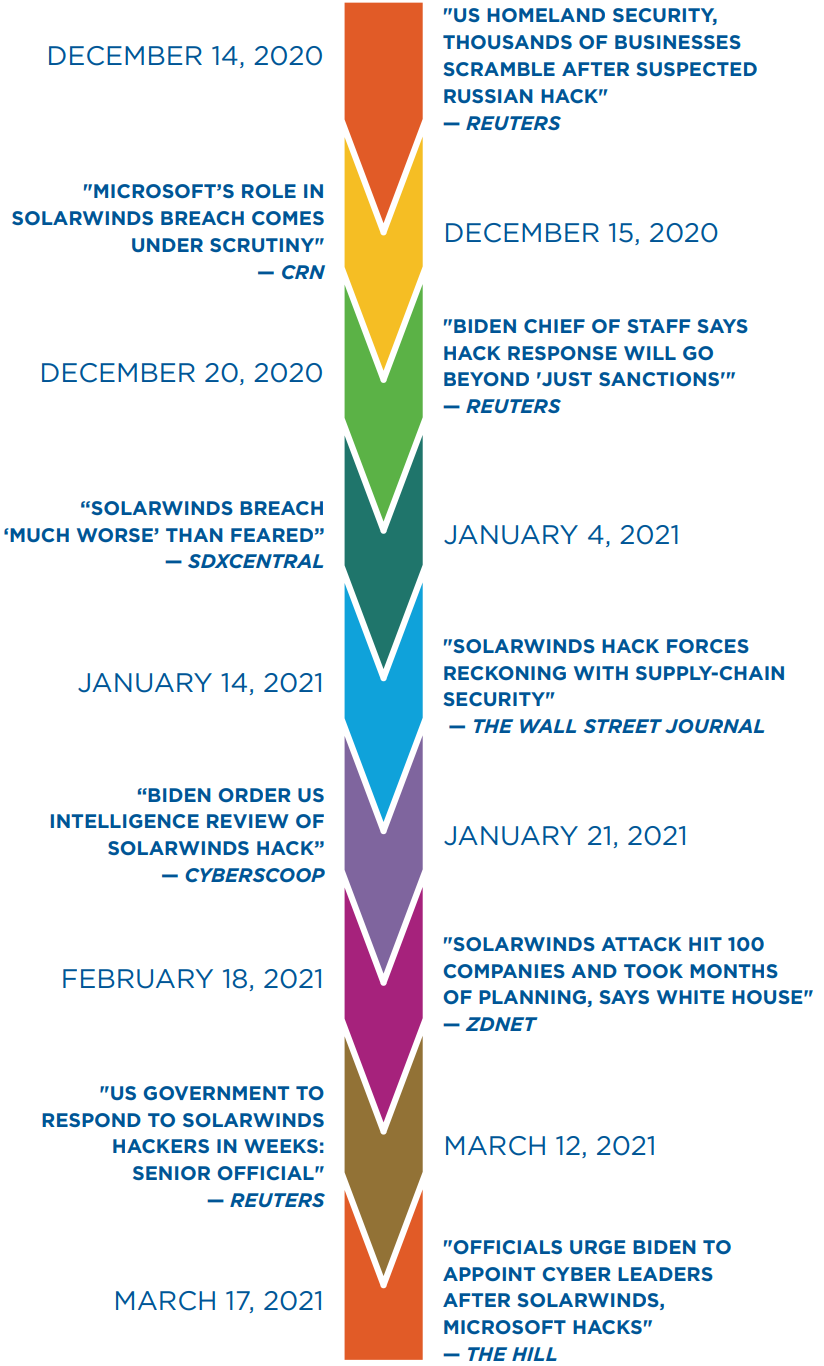
\includegraphics[width=3.4in]{AfterMath-Timeline.png}
        \caption{Source: \cite{BrokenTrustHerrEtAl} }
        \label{fig:AfterMathTimeLine}
    \end{figure}
\subsection{Lessons Learned}

\section{Conclusion}
%key findings, recommendations, future implications, and limitations.


Conclusion text here.

\section*{Citations}


\begin{thebibliography}{}
\bibitem{Microdoft2024NOBELIUM} Microsoft, ``Nation State Actors Midnight Blizzard,'' \emph{Microsoft Security Insider}, Jan. 25, 2024. [Online]. Available: \url{https://www.microsoft.com/en-us/security/security-insider/threat-landscape/midnight-blizzard}. [Accessed: Sept. 29, 2025].
\bibitem{MITREFirstNOBELIUMAttack} MITRE, ``Operation Ghost (Campaign C0023),'' \emph{MITRE ATT\&CK}. [Online]. Available: \url{https://attack.mitre.org/campaigns/C0023/}. [Accessed: Sept. 29, 2025].
\bibitem{MicrosoftDeepDiveSOLORIGATE} Microsoft Cyber Defense Operations Center and Microsoft Threat Intelligence, ``Deep Dive into the Solorigate Second-Stage Activation: From SUNBURST to TEARDROP and Raindrop,'' \emph{Microsoft Security Blog}, Jan. 20, 2021. [Online]. Available: \url{https://www.microsoft.com/en-us/security/blog/2021/01/20/deep-dive-into-the-solorigate-second-stage-activation-from-sunburst-to-teardrop-and-raindrop/}. [Accessed: Sept. 29, 2025].
\bibitem{CoreTech2022Motivations} CoreTech Staff, ``6 Motivations of Cyber Criminals,'' \emph{CoreTech Blog}, Mar. 3, 2022. [Online]. Available: \url{https://www.coretech.us/blog/6-motivations-of-cyber-criminals}. [Accessed: Sept. 29, 2025].
\bibitem{HakalaMelnychuk2021RussiaCyberStrategy} J. Hakala and J. Melnychuk, *Russia’s Strategy in Cyberspace*, NATO Strategic Communications Centre of Excellence, Riga, Latvia, Jun. 2021. [Online]. Available: \url{https://stratcomcoe.org/cuploads/pfiles/Nato-Cyber-Report_11-06-2021-4f4ce.pdf}. [Accessed: Sept. 29, 2025].
\bibitem{NCSC2021FurtherTTPsSVR} National Cyber Security Centre (UK), ``Advisory: Further TTPs Associated with SVR Cyber Actors,'' May 2021. [Online]. Available: \url{https://www.ncsc.gov.uk/files/Advisory-further-TTPs-associated-with-SVR-cyber-actors.pdf}. [Accessed: Sept. 30, 2025].
\bibitem{BrokenTrustHerrEtAl} T. Herr, W. Loomis, E. Schroeder, S. Scott, S. Handler, and T. Zuo, *Broken Trust: Lessons from Sunburst*, Atlantic Council, Scowcroft Center / Cyber Statecraft Initiative, Mar. 2021. [Online]. Available: \url{https://www.atlanticcouncil.org/wp-content/uploads/2021/03/BROKEN-TRUST.pdf}. [Accessed: Sept. 30, 2025].
\bibitem{GAOSolarWindsExchange} U.S. Government Accountability Office, *Cybersecurity: Federal Response to SolarWinds and Microsoft Exchange Incidents*, GAO Report No. GAO-22-104746, Jan. 2022. [Online]. Available: \url{https://www.gao.gov/assets/gao-22-104746.pdf}. [Accessed: Sept. 30, 2025].
\end{thebibliography}
\vspace{12pt}
\color{red}
IEEE conference templates contain guidance text for composing and formatting conference papers. Please ensure that all template text is removed from your conference paper prior to submission to the conference. Failure to remove the template text from your paper may result in your paper not being published.

\end{document}
About
About us
Careers
Blog
Solutions
For business
For universities
For government
For publishers
Customer stories
Learn